% !TeX spellcheck = en_GB
% !TeX spellcheck = en_US 


\chapter{Experimental set-up}

In this chapter we will present the experimental set-up used, given a special section to  the Nanodroplet generations, the doping process and the data acquisition system. A  sub-chapter is also dedicate to the single shot correlation data acquisition system tested specifically to this Master`s project.
The apparatus we worked with is part of the the  group of Molecule and Nanophysics at the University of Freiburg, Germany, and was calibrated and used for the experiments in \cite{schomas_compact_2017} and \cite{heidenreich_charging_2016}.

In figure XXX an sketch of the apparatus is shown. From left to right; The source chamber where the  ultra cold molecular beams are produced, the central chamber or "doping chamber" where the beam gas is doped via pick up process using a gas doping cell or a diffuse oven for alkaloids where gases or thermally vaporized solids and using as dopant, the last  chamber or "detection chamber" combines a VMI - TOF detection system and a  Langmuir taylor (LT) detector.
To generate the nano plasmas the apparatus was Used in two different institutions, at the Max Plank Institute for Nuclear Physics in Heidelberg and the Extreme light institute (ELI) in Szeged, Hungary, because of the special laser systems can be provided in there.

The following sections describes the essential components of the apparatus, taking special attention to the new Triggering systems implemented to correlate the VMI and TOF signals in the last part of the project.  The structure where compacted to a length of about 240 cm long, each chamber has attached its own turbo pumps with  pre-vacuum pumps and are separated by valves and skimmers. On one hand, this enables to manipulate the vacuum in an independent way and control the targets in the "detection chamber", on the other hand a allows an optimum adaptation of the suction power of the pumps to the gas load of the individual chambers as wheel as to ventilate and open, without having to disturb the entire system.

\section{Source chamber}

The Source chamber consists of a 6-way CF vacuum chamber, with a 2-stage cryostat power a cold-head that can be cooled down to 9K, located in entrance of the chamber, parallel to the floor with an attached conical nozzle for the gas expansion process. The cooling capacity of the cryostat  consists of a copper tube, into which pre-cooled helium is introduced. It can be adjusted by operating two heating resistors in combination with a sensor diode for temperature measurement and a PID controller. Controlling the resistor current the temperature at the end of the nozze can be keeping it stable. The conical nozzle used to generate the atomic beam is the standard used in the research group on Nanoplasma reasearch directed by Prf, frank Steankeirmeyer at Freiburg University.  It is made of copper and has a platinum plate on front with a hole of 5$\mu m$ of diameter for $He$ experiments and 15$\mu m$ for $Ne$ gas clusters. The diameters where choseen in order to follow the Size dependence of the \textit{Hagenas} "law",  which together with the adjustable gas pressure and the nozzle temperature regulates the flow.
The cold head-nozzle arrangement are connected to the chamber via a self-made x-y manipulator,  with a thermally insulating rubber? ring, which allows a beam adjustment in relation to the other components in the setup with out braking the vacuum. At the bottom of the chamber an "Agilent" turbo pump of $1800 L/s$ capacity is attached to a pre-vacuum scroll pump as exhaust.
A skimmer with a diameter of $400\mu m$ is located in front of the effusive jet, sorting the gas beam not just by it size but also by its velocity vectors and allowing just those beams with direction to the further vacuum chambers. To adjust the nozzle optimally to the skimmer,it is connected to an x-y displacement unit and can be aligned from outside the vacuum chamber. To prevent the small opening of the nozzle from clogging over time, high-purity helium 6.0 (99.9999$\%$ purity) and Ne 5.0 (99.999$\%$ purity)  is used and can also be used outside of the measurements ensures a constant gas flow through the nozzle. At this extreme temperatures this prevents that any impurity in the gas bottle can  condensate, blocking the nozzle or changing the conditions of the clusters production. 

\section{Dopping chamber}

As explained in the chapter above, the Doping takes place by inelastic impacts with atoms from the gas phase, referenced as the pick-up thecnique. In this experiment we doped with both metals and noble gases, and two different methods of doping are used: Metals are heated in evaporated phase in a oven, while gas dopant yield in a Gas doping cell entered the vacuum chamber through a needle valve. on the next section we will explain the elements of the dopping cham,ber and its most important characteristics used.

The oven chamber is conected after to the Source chammber via the skimmer, it is also a 6-way CF vacuum chamber, with a turbo pump  on bottom, connected to it own pre-vacum scroll pump. On the sides the flanks allows a cold trap not used in this experiment, on the other side  the flank that permit connection to the oven and the vacuum sensor. The Skimmer is made of Niquel??, a very thin metal easy to bend, so in order to prevent stronf pressures diferrence in the chamber that can modify the skimmer, a bypass is conected between the two chamber using a stainlees steel flexible hose.  
An internal stand is welded to the front of the chamber and aligned with the skimmer. This stand supports the Chopper, the gas dopping cell and the oven.
In the front the rail the choppers is located.  It is an steel  disk with three notches uniformed located,two photocell around the bottom of the disk reads the position of the bottom notches so the upper one can be positioned right in front the skimmer. In this way, when the disk rotates the beam can pass or its block by the disk  in a controlled way.  

After the chopper, there is the Gas Dopping cell, a circular flat metal base with a self modified KF hose. The base makes the base cell have a matching patter so the hose can be easy put and remove with out losing the alignment. The stainless steel flexible hose has two $5mm$ hole (one in front and one opposite to it, some cm up the base) alligned to the skimmer so the gas bean can go thought. The hose is fix to the base and goes to the top of the chamber where it is connected to a "swaglog" niddle valve that allows to control the gas flux for doping the beam. A Pfiffer CMR375 Capacitive sensor is located after the niddle valve so a better control of the pressures, ans so of the number of dopants in the cluster can be achived. This bendable construction allows not just to remove the doping cell with out difficulty but also to fit it on the top with out depending on a fix way to located the top plank, in this way there is room for maniouver and the construction is faster.

Finally at the end of the rail lies the Oven. As shown in fig XXX the oven consist on a patterned base (similar to the gas cell) that can  move a few $mm$ on $x-y$ plane. Over it, a metal cylinder with 4 heating cartridges holds a movable crucible in the center that contains the dopant sample, this movable container is set down by a rod that comes from the top of chamber after a valve. Both, the stove and crucible have holes (a conical entrance of $40mm$ diameter and $3mm$ diameter respectively) that allows the pass of the gas beam and are aligned to the beam pad, in this way  the passing Atomic beam takes dopants via collisions with vaporized sample material.

One important advantage of this new oven design done by \textit{Dominic Schomas},  is that the dopant can be change with out braking the vacuum, it was test in this experiments and prove to be useful saving time and effort. To control the temperature of the oven a temp sensor is fix in the stove, and the resistors current is manage by a PID controller allowing a stable temperature during the experiment. The maximal temperature reached was $450^{\circ}c$,  enough to creates the gas phase for the potassium K and calcium Ca used in this experiment as shown in the table XXXX. Finally there is an  extra skimmer of diameter XXX fixed to a valve between the connection of the doping chamber and the detection chamber that helps to avoid the disperse beams or an overflow from one chamber to the other.

In addition to the doped gas nano droplets, effusive gas is also released from the dopant chamber into the detector chambers through a "swarlog niidle valve" and can be ionized and detected there. This disperse gas was pour in directly on the chamber or filtered by diffusive atoms going out of the oven and passing across the second skimmer once the choppers is close. This atomic gases where added for calibration of the detectors and background reduction allowing just one gas at a time.

\section{Detection chamber}

As mentioned, the detector chamber is connected to the Oven chamber through a valve and a skimmer. The detector chamber contains a newly developed Velocity-Map-Imaging
spectrometer on top, a time-of-flight mass spectrometer on bottom and a LT detector on front. On this section we will give a brief presentation of  the VMI and the TOF used for this experiment, taking spacial interest on the new Triggering process that allows to detect single nanoplasma explosions. 

\subsection{Velocity map imaging VMI}

The VMI detector used in this experiment is detail in \cite{schomas_compact_2017}, this construction basically follows the standard geometry of Eppink and Parker\cite{eppink_velocity_1997}. Its composed by three electro lenses (repeller, lens and extractor) that focuses the ions or electrons on a $86,6mm$ (effective area) diameter Micro channel plates (MCP) arrange. This detector set is basically  two MCP´s superposed,  rotated to each other and a phosphoscreen (PS) layer of same diameter facing the top plank of the chamber with a Ca-fluoride glass of $1mm$ thick. A, external CCD camera is focused to the PS. 

\begin{table}[]
\centering
\begin{tabular}{|l|l|l|l|}
\hline
\rowcolor[HTML]{EFEFEF} 
VMI & Repeler & Extractor & Lens  \\ \hline
X1  & -2430   & -1940     & 3500  \\ \hline
X3  & -7290   & 5820      & 10500 \\ \hline
Ion & 2430    & 1940      & 0     \\ \hline
\end{tabular}
\end{table}

The voltages applied to the MCP and PS determine the brightness of the final pictures of the ions, so in general just one set of voltages were use, around $1400V$ for the MCP and $4000V$ for the Ps. The achievable energy acceptance for this stack is  $34eV$ for a the VMI setting 1 and $270 eV$ for the X3 settings. The VMNI have a resolution of $\bigtriangleup E / E\leq 4\%$ \cite{schomas_compact_2017}. The camara used in the experiment was a Basler  acA1920-155um focused on the PS.

\begin{figure}[hbtp]
\label{img:mcp cut}
\centering
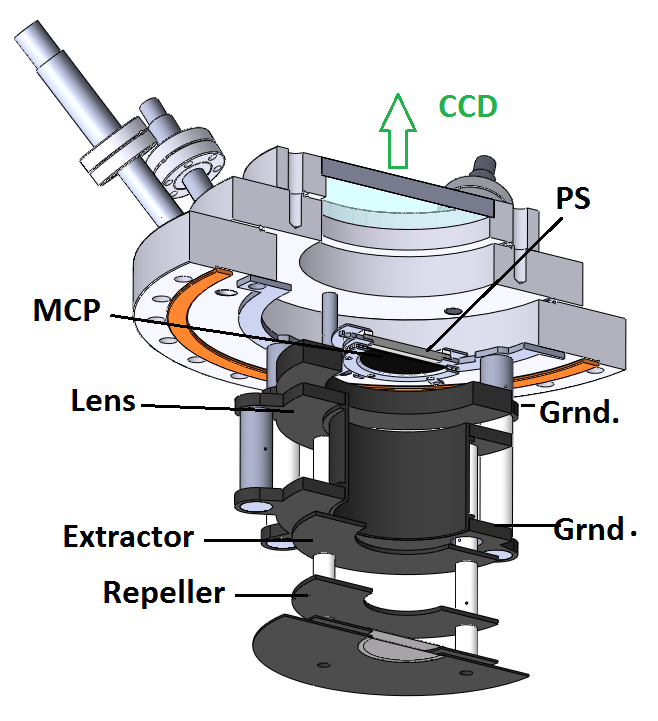
\includegraphics[width = 8 cm]{../Images/MCP cut.png}
\caption[MCP sketch cut]{Sectional cut view of the CAD model of the spectrometer setup. On black  the electrodes and the white the Polyether ketone (PEEK) isolators. On orange, the cooper ring and on blue the top window facing the cCCD camera
}
\end{figure}

On fig \ref{img:mcp cut} we present a view of the model of the VMI used in this experiment, From botom to top, the structure of the electrodes consists of two repeller electrodes separated by a few millimetres with circular openings on which a fine mesh copper grid is applied, an aperture electrode as extractor, another aperture electrode which is held at ground potential and then from the extended lens electrode with the following second ground electrode. At top  the MCP-PS arrange (o black the MCP and on gray the PS) facing the center of the window instales in the top blanck of the chamber. Around thewwindow there are three conections that allows the voltages for the electrodes and the cables are carefully arrange around tthe structure to avoid discharges or even disturb the uniform electrical field.

The openings of the repeller (on bottom in bluish color) electrodes allow the use of these electrodes as well as extractor electrodes for a TOF spectrometer. In simultaneous operation of the VMI and the TOF spectrometer, the glued grids prevent mutual field effects of the two spectrometers.  The repeller and extractor are grade 2 titanium and the lens is stainless.

\section{Time of flight spectrometer}

The Time of fligth (TOF) spectrometer used was based on the desing by Wiley and McLaren \cite{wiley_timeflight_1955}. As it names reefers, the TOF mass spectrometer relates the time that a particle on an electric field requires to reach certain distance with its mass,  when atoms and molecules are photoionized,  they pass through an electrostatic acceleration field and are registered in a detector after crossing a field-free flight path. Based on the flight time the ratio $m/q$ of a particle can be determined as:

\begin{equation}
t-t_{0}=a\sqrt{\frac{m}{q}}
\end{equation}

Where $a$ is a experimental factor depending of the flight distance, electric fields and material of the setup,  $m/q$ is the relation mass - charge, $t_{0}$ is the time ionization time (given by the laser )and $t$ is the time of flight.

The ions creation takes place in the aperture between the repeller and extractor electrodes. Behind the extractor electrode there is a further aperture electrode, which is held at zero potential and thus generates a pre stablish flight route with a defined field, grids are glued to the openings of the electrodes to prevent the propagation of the fields through the orifices in the electrodes. The repeller electrode is set to a positive potential and the extractor to a negative potential. The resulting electric field accelerates the ions through the openings in the flight tube, on which grids are mounted on both sides to keep the drift path free of field.
Once the coulomb explotion takes places, the ions are accelerated by the electric field of the repeller and then fly through a field-free drift path to the detector. This allows a complete mass spectrum to be recorded within a few microseconds in a single measuring step \cite{mobius_time--flight_2016}.

\begin{figure}[hbtp]
\label{img:tofcup}
\centering
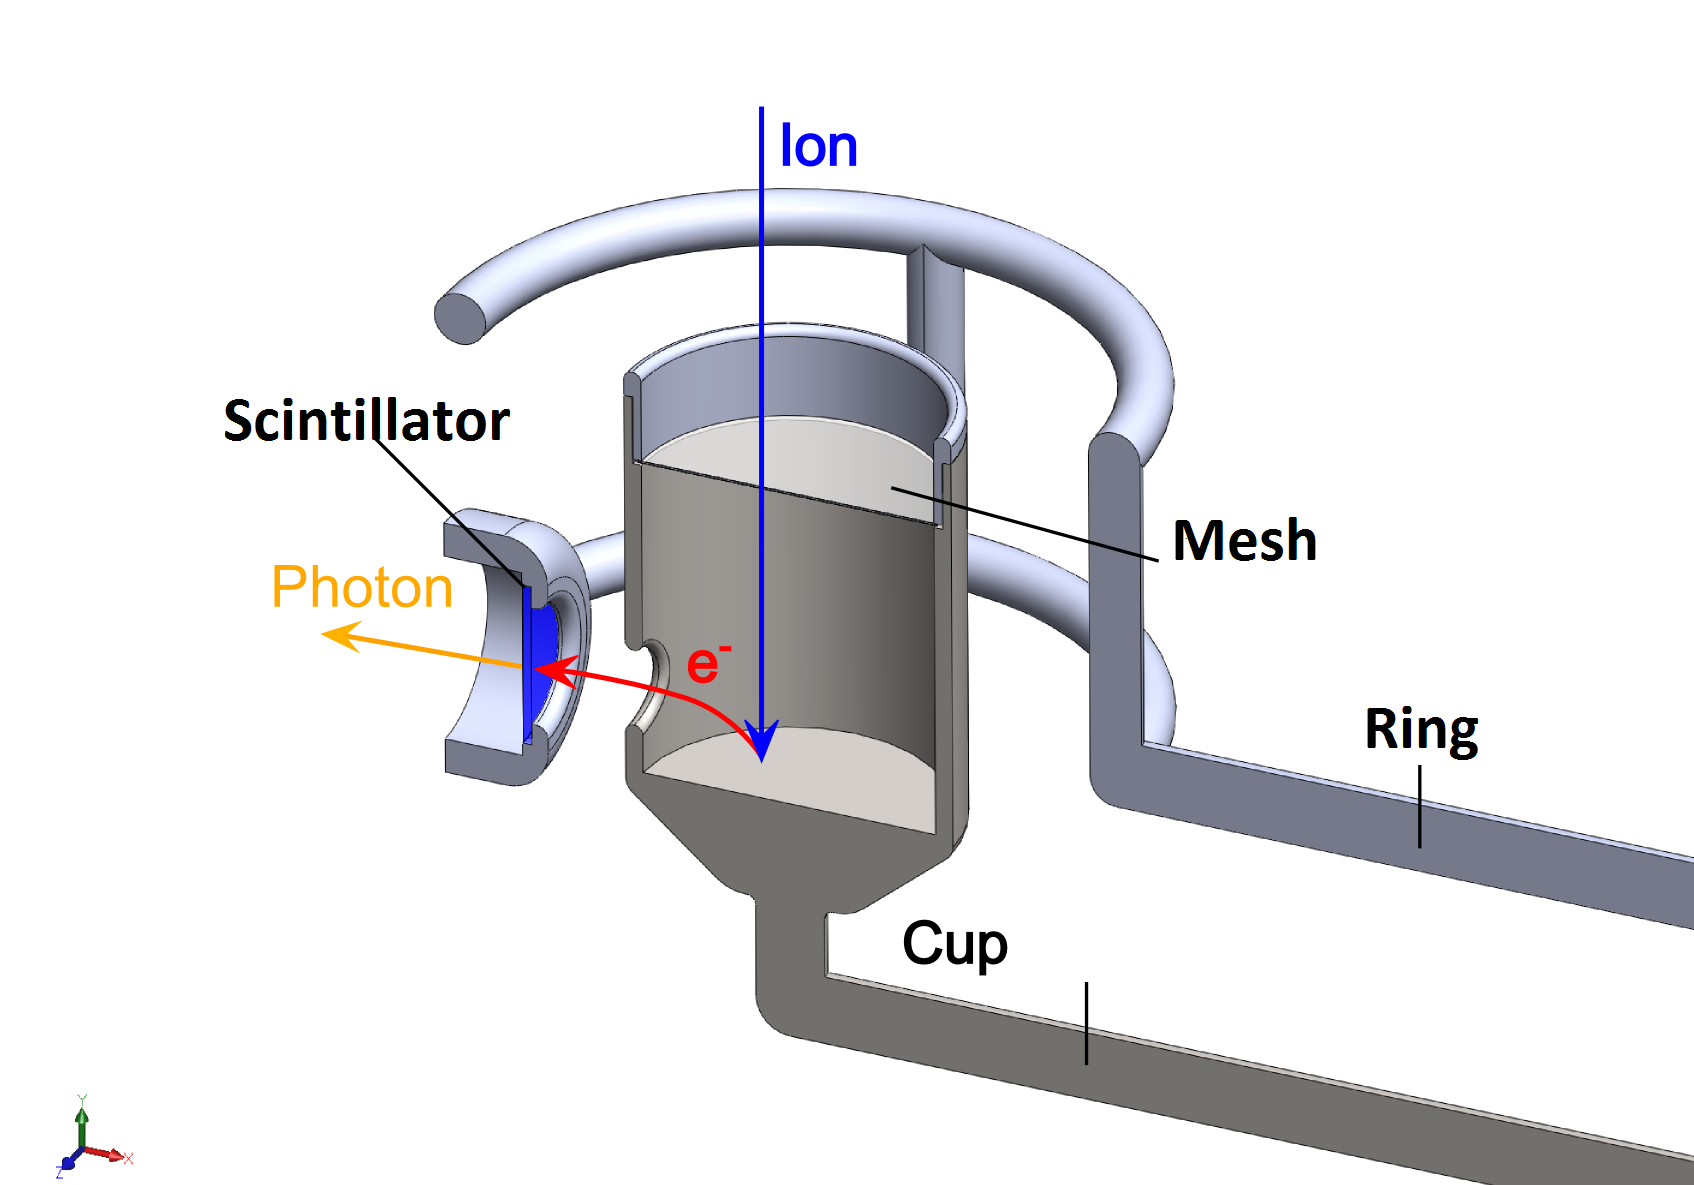
\includegraphics[width = 10 cm]{../Images/Cup scintillator.png}
\caption[TOF cup]{Illustration of the functional principle of a Daly detector.}
\end{figure}

The flying Ions finally are detected by a  Daly detector \cite{daly_scintillation_1960}. It consists of a cup, a grid and a ring. The cup lies on negative high voltage while the ring on positive. The ions from the repeller pass trough the field free tube corrected by a drift electrode.  Since in the direction of the hole the potential for electrons drops sharply, the ring electrode generates an electric field, which directs the ions into the cup. The ions that pass the  the grid at high speed hits on the bottom of the cup, they generate some electrons, which are transmitted through a small hole in the bottom and then in a scintillator Eljen thechnilogy(EJ-204) flashes some photons in the process. These ligth is detected in a Hammamatzu r-647 photomultiplier. The voltage output of the photomultiplier is controlled by a fast analogue-to-digital converter, and its used at a $900V$ voltage. The cup and the drift-scintellator  tube where set at high voltages,  $-17000V$ and $-4000$ respectively.

\section{Lt detector}

The Langmuir-Taylor detector (LT detector)  chamber consists of a small CF40-6-way chamber. The detector consists essentially of an annealing filament, which is located between two planar round electrodes. The Operating Principle of an LT-Detector 
is based on surface ionisation by the tunnel effect \cite{delhuille_optimization_2002}. For the annealing filament is typically used  rhenium, platinum or tungsten, as this is the most common due its comparatively high electron work function. With high voltages, the wire reach high temperatures, as a consequence, a passing neutral atoms is ionized, releasing an electron into the wire. The resulting ions is attracted by the negative electrodes around the wire generating a current. The ionic current generated at the electrodes is proportional to the number of ionized atoms and is measured using a pico amperimeter.
The LT chamber is connected to the VMI chamber via an orifice plate and is used mainly as a beamdump and to align the detector. The most current generated on the chamber the most atoms are passing through the  hole, so we can be sure that the beam pad is in the detection area.

\section{Camera and trigger protocol}

The aim of this master thesis was to achieve individual data for single shots nanoplasma explosion in the VMI and TOF. The advantage of this correlation is the ability of threat the data in a separate way, to reduce the background and achieve  properties on the coulomb explosion that are not possible when averaged data is used.

Two methods were developed for this work. A first approach was done using a software trigger for the CCD camera and the oscilloscope for the TOF, an Acqiris Card CC103. Using LabView, an external clock (a RasberryPi 3) was triggered by the laser, the beginning of the explosion,  at the same time, it software-trigger the camera and oscilloscope programs to start the acquisition. Having all the data acquire in the same software would allow to sort the data online and reduce the storage needed to the experiment. The Labview program was tested unsuccessfully for the data acquisition rate needed in ELI $100KHz$, the main problem was, that when an software-triggering scheme is used,  extra delays are applied due the operating system and the communication protocols, so even the data were acquire at the same time the delays in at saving  it in the hard drive made impossible to correlate the signals.

Based on that same idea, a second approach was used. As alternative of the software triggering a hardware triggering was used. The laser triggers a delay generator that at the same time triggers the oscilloscope, a R&S RTO2000 with bandwidth of 600MHZ to 6GHz,  and the camera. Two facts had to been taken into account, first, the minimal exposure time of the camera is $34\mu s$. Second, the timing between the camera receiving the trigger and the real start of the acquisition is not negligible as it is for the oscilloscope. The camera took between $5-6 \mu s$ to start after the trigger was send. To solve this problem the triggering scheme in fig \ref{fig:triggers}.
\begin{table}[]
\label{tab:delaystriger}
\begin{tabular}{ll}
\multicolumn{2}{c}{List delays}                                          \\ \hline
\multicolumn{1}{|l|}{Channel} & \multicolumn{1}{l|}{Set to:}    \\ \hline
\multicolumn{1}{|l|}{A}                & \multicolumn{1}{l|}{$=T+0$}       \\ \hline
\multicolumn{1}{|l|}{B}                & \multicolumn{1}{l|}{$=T+1\mu s$}     \\ \hline
\multicolumn{1}{|l|}{C}                & \multicolumn{1}{l|}{$=B or B+6\mu s$} \\ \hline
\end{tabular}
\end{table}

A delay generator (Stanford Research Systems MD DG335) recive the laser trigger (100KHz) channel B and C where connected to the oscilloscope to channel 1 and 2 respectively, and channel A was connected to the pin 1 (trigger) on the camera. Due the limitation of exposure time of the camera, we can not identify a single laser shot with it. Table \ref{tab:delaystriger} shows the delays used in the experiment, where $T$ is the original laser trigger and  A,B and C are the channels in the delay generator. In this way, it can be shown in fig, that the oscilloscope can "see" each of the laser shots individually but the camera will see at least 3 shots, but fortunately, not each laser shot generates signal, as show in the next chapter in general just $10 to 20\%$ of the laser short ignites a plasma explosion, this mean that most of the pictures will have no signal, rare cases will have two or more explosion and the pictures with actual signal will contain just one  explosion in the VMI that can be correlated to its individual TOF signal. 

\begin{figure}[hbtp]
\label{fig:triggers}
\centering
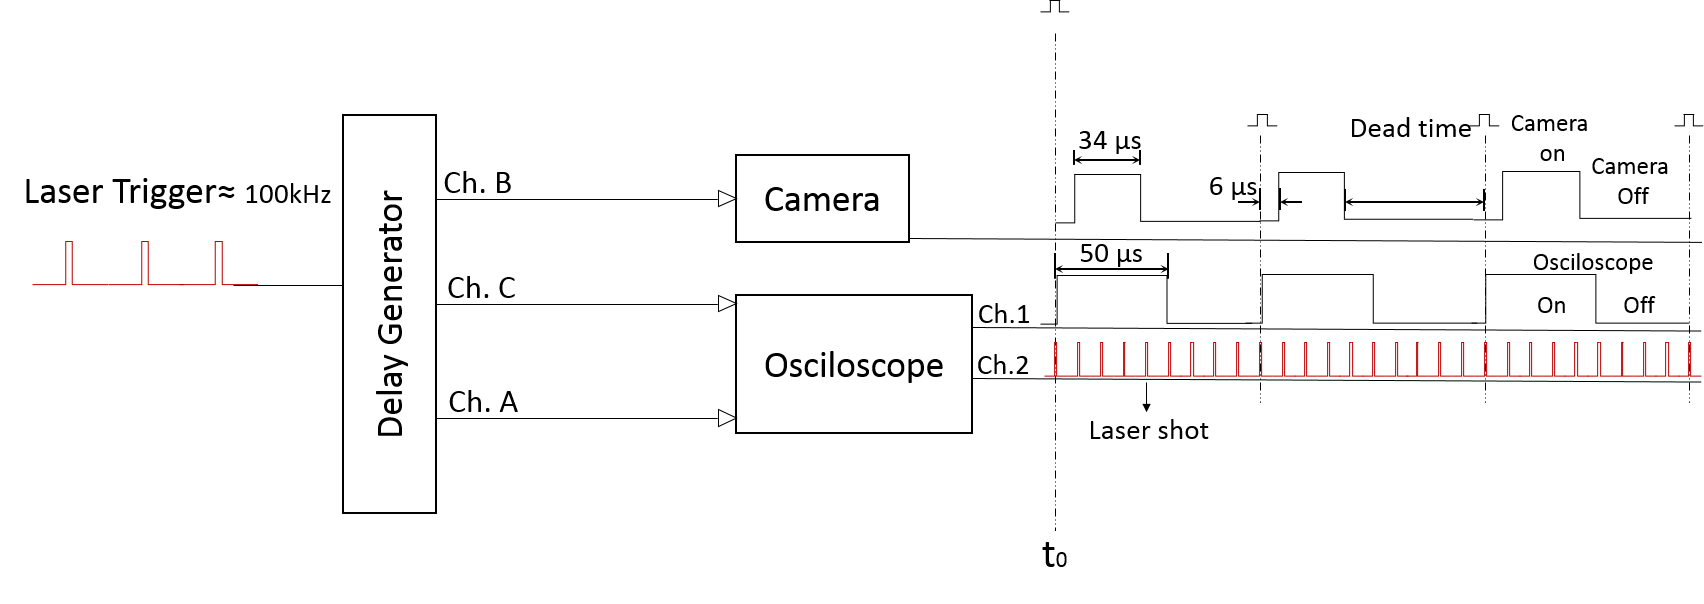
\includegraphics[width = 14 cm]{../Images/Trigger scheme.png}
\caption[Trigger Scheme]{Scheme of the trigger system used.  }
\end{figure}

In Fig \ref{fig:triggers}, we show the Trigger scheme used in the experiment. The oscilloscope and camera are triggered by the delayed channel B. The oscilloscope is set to $50\mu s$ and the camera to the minimal exposure time. So the camera and oscilloscope sees the same trigger, the oscilloscope will record at least 5 laser shots, but the camera because starts later just can see three as shown. The pictures are saved in the memory RAM of the computer so the dead time after the camera is off is mandatory to give the operative system enough time to save the data on disk and don't full the Ram. A small improvement in this system can be done if we trigger the camera with B and the oscilloscope with C, so both apparatus can start almost at the same time and no corrections needs to be done. Each of the data set are saved with a unique label that will help to correlate the data after. Once a explosion is found in the VMI pictures, we check in its corresponding TOF that it have just one signal in all five laser shots, so we can be sure that picture correspond to a single coulomb explosion, in case more than one signal is found, this picture is discard. 




